
%\begin{table}
%	\begin{tabular}{ C{1.5cm} | C{0.7cm} C{2cm} C{1.5cm} C{1cm} C{1cm} C{1cm} C{2cm} C{2cm} | C{2cm} }
%		& age & MyasteniaGravis & arthritis & c3level & c4level & hematological & skinrash & sledai2kInferred & SDI \\
%		\hline
%		Visit 0 & 44.23 & 0 & 1 & 119 & 9 & 0 & 0 & 12.0 & 0 \\
%		Visit 1 & 44.63 & 0 & 0 & 96  & 7 & 0 & 0 & 2 & 0 \\
%		Visit 2 & 44.77 & 0 & 1 & 85.42 & 6 & 0 & 0 & 2 & 0 \\
%		Visit 3 & 44.98 & 0 & 1 & 76 & 6 & 0 & 0 & 2 & 0 \\
%		Visit 4:& 45.58 & 0 & 0 & 76 & 6 & 0 & 0 & 1 \\
%	\end{tabular}
%\end{table}

\begin{frame}{Lupus disease prediction}

	The \textbf{goal} is to predict whether a patience will develop the lupus disease in the near future given its medical history.
	\vspace{2em}\\
	Dataset:
	\begin{itemize}
		\item Gathered by the ``Lupus Clinic'', Reumatologia, Università Sapienza, Rome.
		\item Patients have a different number of visits.
		\item Visits are not equally spaced over time.
		\item Small dataset ($\sim100$ negatives, $40$ positives).
	\end{itemize}

\end{frame}

\begin{frame}{An example of a record of a patience}
\begin{table}[H]
	\centering
	\begin{tabular}{ C{2.5cm} | C{1cm} C{1cm} C{1cm} C{1cm} C{1cm}}
		& Visit 0 & Visit 1 & Visit 2 & Visit 3 & Visit 4 \\
		\hline
		age & 44.23 & 44.63 & 44.77 & 44.98 & 45.58 \\
		MyasteniaGravis & 0 & 0 & 0 & 0 & 0 \\
		arthritis & 1 & 0 & 1 & 1 & 0 \\
		c3level & 119 & 96 & 85.42 & 76 & 76 \\
		c4level & 9 & 7 & 6 & 6 & 6 \\
		hematological & 0 & 0 & 6 & 6 & 6 \\
		skinrash & 0 & 0 & 0 & 0 & 0 \\
		sledai2kInferred & 12 & 2 & 2 & 2 & 0 \\
		\dots & \dots & \dots & \dots & \dots & \dots \\
		\hline
		SDI & 0 & 0 & 0 & 0 & \textbf{1}\\
	\end{tabular}
\end{table}	
\end{frame}


\begin{frame}{Numerical results for the lupus disease prediction}

\begin{figure}
	\centering
		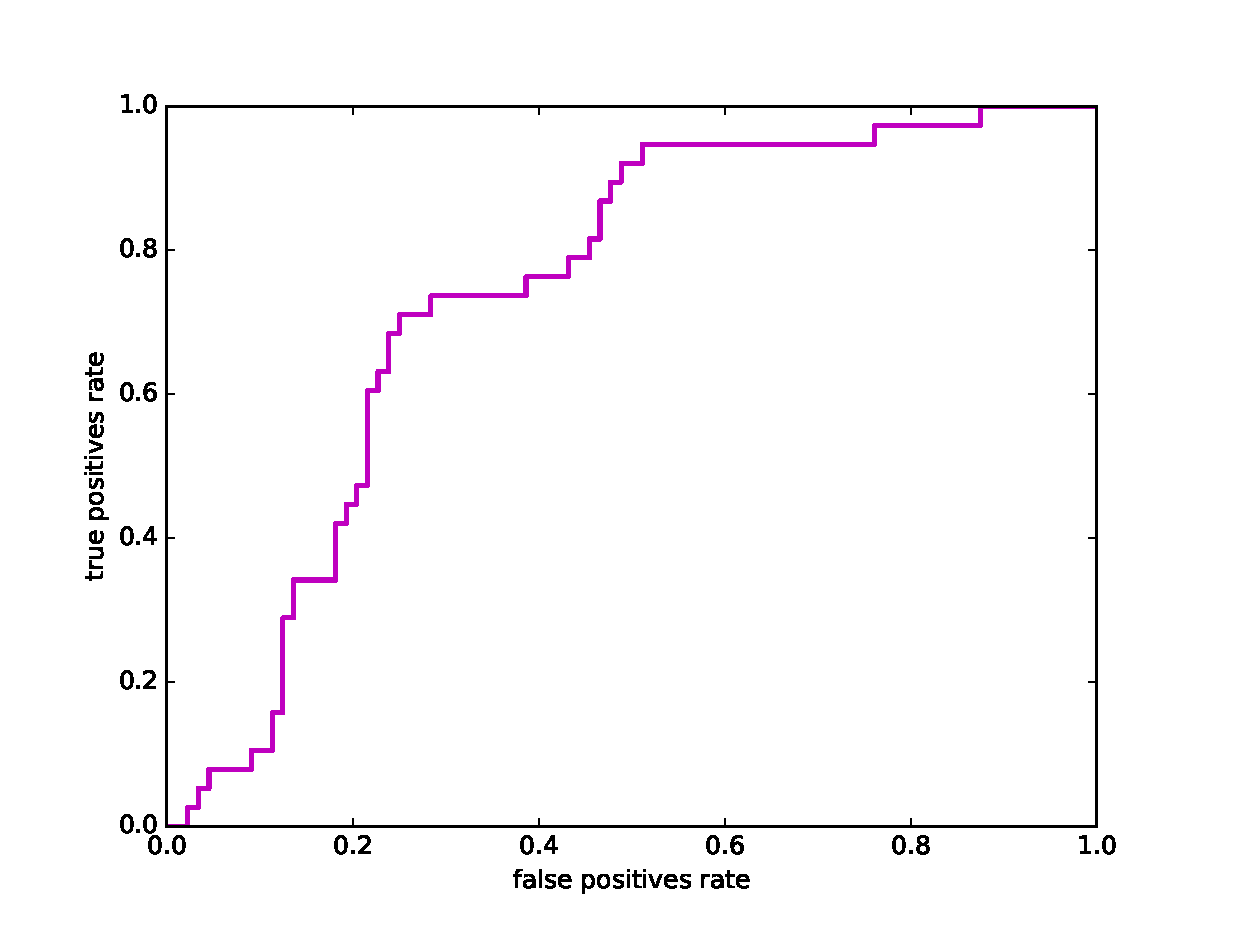
\includegraphics[width= 0.6\textwidth]{plot_roc_lupus_roc_.eps}
		%			\caption{roc curve for models of Line 5 of Table \ref{table:exp_res}.}
		\caption{ROC curve. AUC score is 0.74}
		\label{fig:lupus_roc}
\end{figure}

\begin{itemize}
	\item Results considered promising by medical experts.
	\item Improvable when more data will be available.
\end{itemize}

\end{frame}


 
